\documentclass[tikz]{standalone}
\usepackage{amsmath}
\usetikzlibrary{calc}
\definecolor{bgdark}{HTML}{171D2B}
\definecolor{acc}{HTML}{F7B538}
\definecolor{soft}{HTML}{2A3447}
\definecolor{mut}{HTML}{8FA0BF}
\pagecolor{bgdark}
\begin{document}
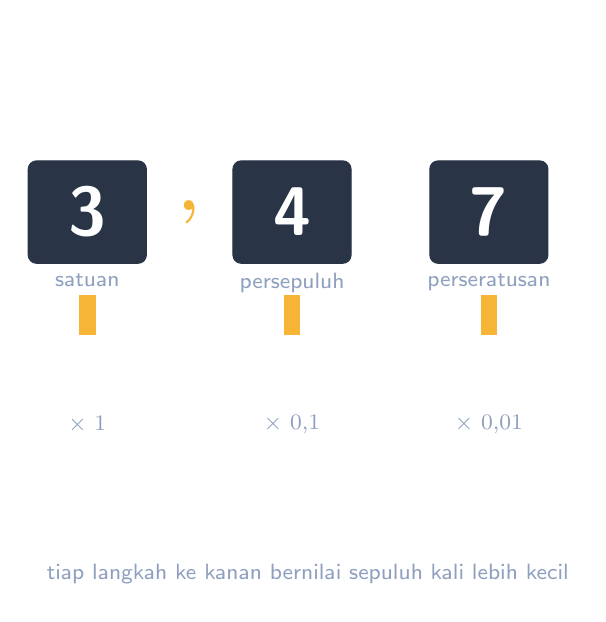
\begin{tikzpicture}[x=1cm,y=1cm,font=\sffamily]
  \tikzstyle{cell}=[draw=soft,fill=soft,minimum width=1.5cm,minimum height=1.3cm,rounded corners=3pt]
  \tikzstyle{lbl}=[mut,font=\footnotesize\sffamily]
  % title
  \node[white,font=\Large\sffamily\bfseries] at (4.6,3.6) {3{,}47 dibaca per kolom};
  % cells
  \node[cell,label={[lbl]below:satuan}] (u) at (1.8,1.6) {\Huge\bfseries\color{white}3};
  \node[acc,font=\Huge\bfseries] at (3.1,1.6) {,};
  \node[cell,label={[lbl]below:persepuluh}] (d) at (4.4,1.6) {\Huge\bfseries\color{white}4};
  \node[cell,label={[lbl]below:perseratusan}] (c) at (6.9,1.6) {\Huge\bfseries\color{white}7};
  % value bars under digits
  \draw[acc,line width=6pt] ($(u.south)+(0,-0.9)$) -- ++(0,0.5);
  \draw[acc,line width=6pt] ($(d.south)+(0,-0.9)$) -- ++(0,0.5);
  \draw[acc,line width=6pt] ($(c.south)+(0,-0.9)$) -- ++(0,0.5);
  \node[lbl] at (1.8,-1.1) {$\times\ 1$};
  \node[lbl] at (4.4,-1.1) {$\times\ 0{,}1$};
  \node[lbl] at (6.9,-1.1) {$\times\ 0{,}01$};
  % expansion line
  \node[white,font=\sffamily] at (4.6,-2.0) {$3{,}47 = 3\times 1 + 4\times 0{,}1 + 7\times 0{,}01$};
  % note
  \node[mut,font=\footnotesize\sffamily] at (4.6,-3.0) {tiap langkah ke kanan bernilai sepuluh kali lebih kecil};
\end{tikzpicture}
\end{document}
